\section{Example cases}
\label{section:cases}

To drive the adapter development and test the software at its current state, two example cases were implemented. The OpenFAST simulation of a single wind turbine, namely the NREL 5MW model \cite{Jonkman:2009}, should be coupled. The first case couples the simulation to a dummy fluid solver. While performing no realistic computations, the dummy is handy to get an insight into the different data structures, mesh setups, and mapping options. The second case couples OpenFAST to OpenFOAM. It can be seen as a first proof-of-principle with a successful data exchange between the tools. However, more work needs to be done to ensure a correct and robust simulation. Both cases are part of the repository on GitHub\footnote{\url{https://github.com/LeonardWilleke/openfast-adapter/tree/main/cases}}.

\begin{comment}
\begin{itemize}
\item Two example cases were implemented to drive the adapter development
\item The OpenFAST simulation of a single NREL 5MW turbine \cite{Jonkman:2009} should be coupled
\item Coupling to dummy fluid solver to test the data exchange
\item Coupling to OpenFOAM to test the mapping with a CFD tool
\item Both cases are part of the repository on GitHub\footnote{\url{https://github.com/LeonardWilleke/openfast-adapter/tree/main/cases}}\\
\end{itemize}
\end{comment}

\subsection{Coupling OpenFAST with a dummy CFD solver}

The reasoning behind this case is to provide a simple and fast way to test different functionalities and gain insight, not to perform realistic simulations. OpenFAST computes a NREL 5MW turbine with a fixed rotor to avoid mesh problems on the moving blades. The fluid solver is implemented as a simple C++ script that calls preCICE to enable the coupling. It creates a mesh that can be used to map data from OpenFAST on it and writes constant values back, but does not perform any calculations. The setup allows to explore the mapping and data exchange.

OpenFAST employs two internal meshes of the turbine surface with different vertices. Force data is stored on one mesh, while the flow velocity is stored on another. Both meshes can be accessed by the C++ API. However, it is also possible to exchange both variables with the velocity mesh and let OpenFAST map the force data to the force mesh internally. Inspired by the coupling setup in \cite{Taschner:2022}, I want to access both meshes and use preCICE for the mapping. This results in the elaborous coupling scheme seen in Figure \ref{fig:dummy:coupling}. In total, three meshes are employed: The Fluid solver has one mesh \textit{Fluid-Mesh} used for both the force and velocity data while the Solid solver (OpenFAST) uses two meshes. \textit{Solid-Mesh-Velocity} is the velocity mesh of OpenFAST, on which the velocity data from the Fluid solver is mapped. \textit{Solid-Mesh-Force} is the force mesh of OpenFAST, from which force data is mapped back to the Fluid solver.

\begin{figure*}[h]
	\centering
	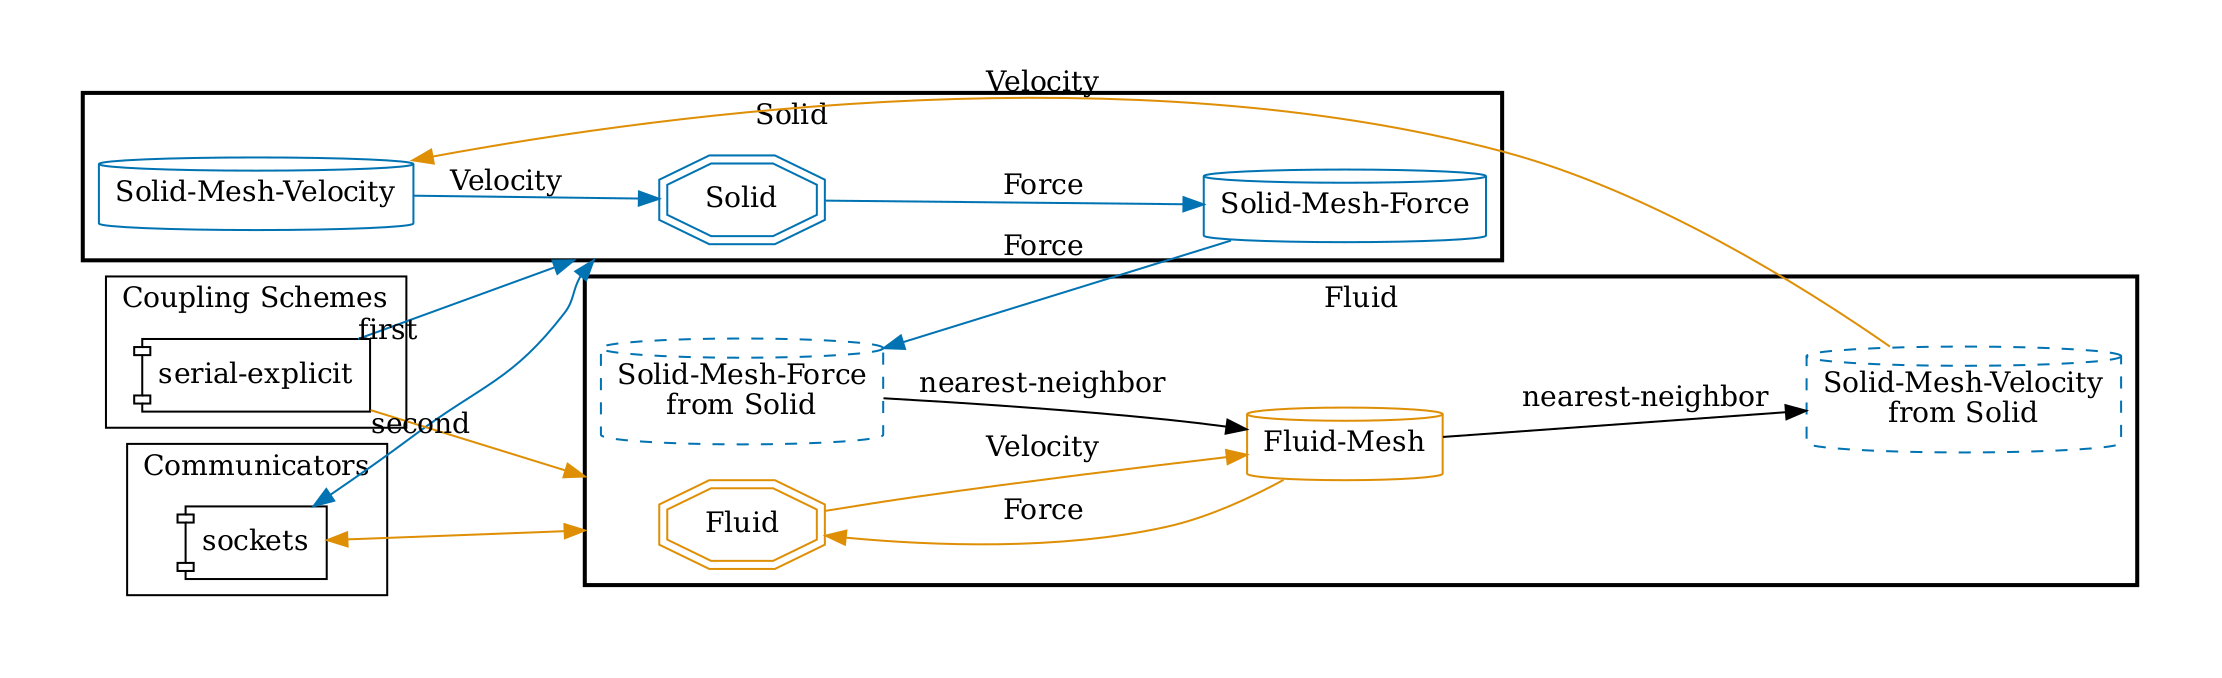
\includegraphics[width=0.9\textwidth]{images/openfast-dummy-coupling-scheme.png}
	\caption{Coupling scheme between OpenFAST, named Solid, and the dummy Fluid solver. The figure was created from the \textit{precice-config.xml} using the \textit{config visualizer tool}\protect\footnotemark.}
	\label{fig:openfast:coupling}
\end{figure*}

\footnotetext{\url{https://precice.org/tooling-config-visualization.html}}

\begin{comment}
Case dummy-turbine
\begin{itemize}
\item Explain the setup
\begin{itemize}
\item Couple OpenFAST to a dummy fluid solver
\item OpenFAST computes a NREL 5MW turbine with a fixed rotor to avoid problems due to the moving mesh
\item Fluid solver is implemented as dummy: No CFD calculation takes place
\item The dummy creates a mesh on which data from OpenFAST is read and writes back constant values
\item Allows to explore the mapping and data exchange
\item Can be used for regression tests in the future (use in challenges)
\end{itemize}
\item Explain the mesh use of OpenFAST
\begin{itemize}
\item OpenFAST has two internal meshes of the turbine surface with different vertices
\item Force mesh: Used to store and compute the surface force
\item Velocity mesh: Used to store and compute the flow velocity
\item Possibility to let OpenFAST map between the two meshes
\item Both meshes can be accessed via the C++ API
\item We want to use preCICE for the mapping
\item A similar coupling setup is employed by \cite{Taschner:2022} who also uses both meshes
\item Maybe add a visualization of the coupling scheme to clarify the mesh use\\
\end{itemize}
\end{itemize}
\end{comment}



\subsection{Coupling OpenFAST with OpenFOAM}

The coupling of OpenFAST with OpenFOAM uses the same coupling scheme as presented in the previous case. However, we are dealing now with 

Case cfd-turbine
\begin{itemize}
	\item Explain the setup
	\begin{itemize}
		\item Couple OpenFAST to OpenFOAM
		\item The coupling scheme and mesh use is identical to the dummy
		\item Now we are dealing with a different mesh on the fluid solver
		\item Main obstacle: The OpenFOAM adapter is not designed to implement a coupling with a solver using the actuator line method. How to map between the line mesh in OpenFAST (Figure )\ref{fig:mesh:fast} and the volume mesh in OpenFOAM (Figure \ref{fig:mesh:foam})?
	\end{itemize}
	\item Explain how the current setup works
	\begin{itemize}
		\item Define a cellSet inside the OpenFOAM domain (Figure \ref{fig:mesh:foam}) to which OpenFAST is coupled
		\item Write the rotor and tower data to this subdomain
		\item Read velocity data from this subdomain
		\item The mapping from line to volume and back is done by preCICE, but probably wrong
	\end{itemize}
	\item How should the turbine be represented in OpenFOAM?
	\begin{itemize}
		\item Volume mesh / cellSet
		\item Surface mesh / patch
		\item ALM implementation (eg with turbinesFoam)\\
	\end{itemize}
\end{itemize}

\newpage
\begin{figure*}[h]
	\centering
	\begin{subfigure}{0.7\textwidth}
		\centering
		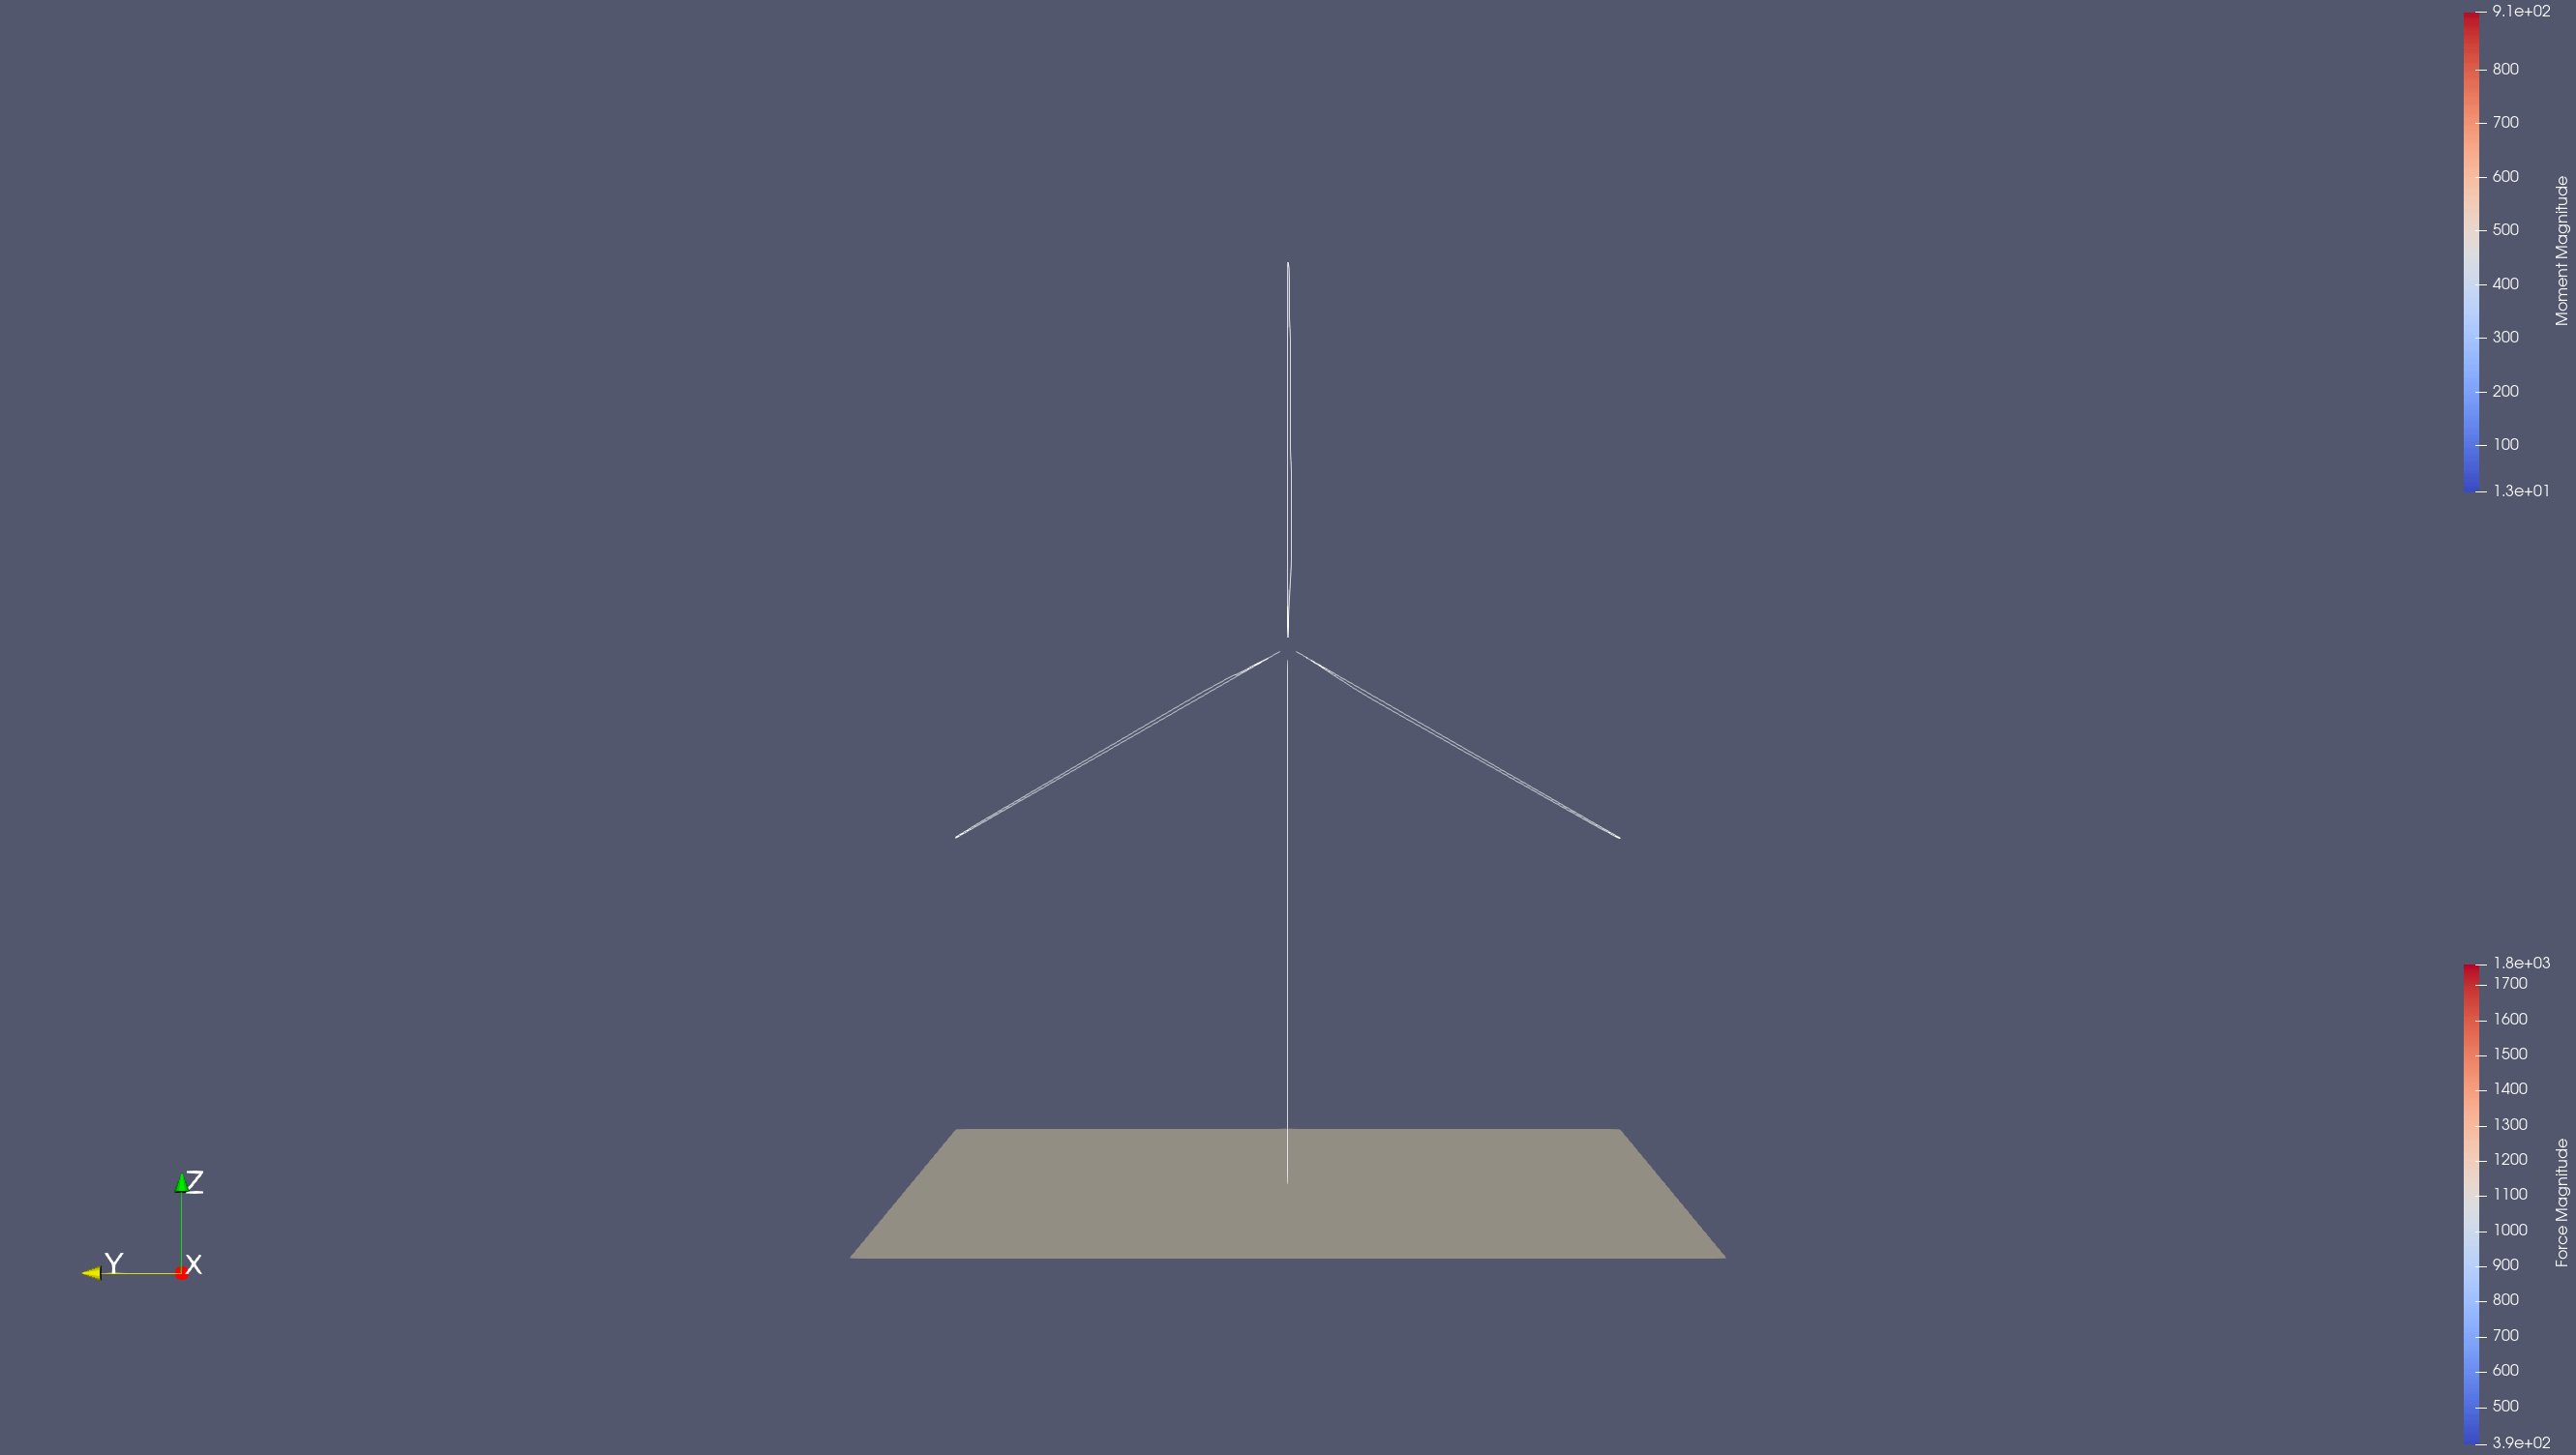
\includegraphics[width=\linewidth]{images/openfast-turbine-mesh.png}
		\caption{Line representation of the turbine in OpenFAST}
		\label{fig:mesh:fast}
	\end{subfigure}
	\vspace{2pt}
	\begin{subfigure}{0.7\textwidth}
		\centering
		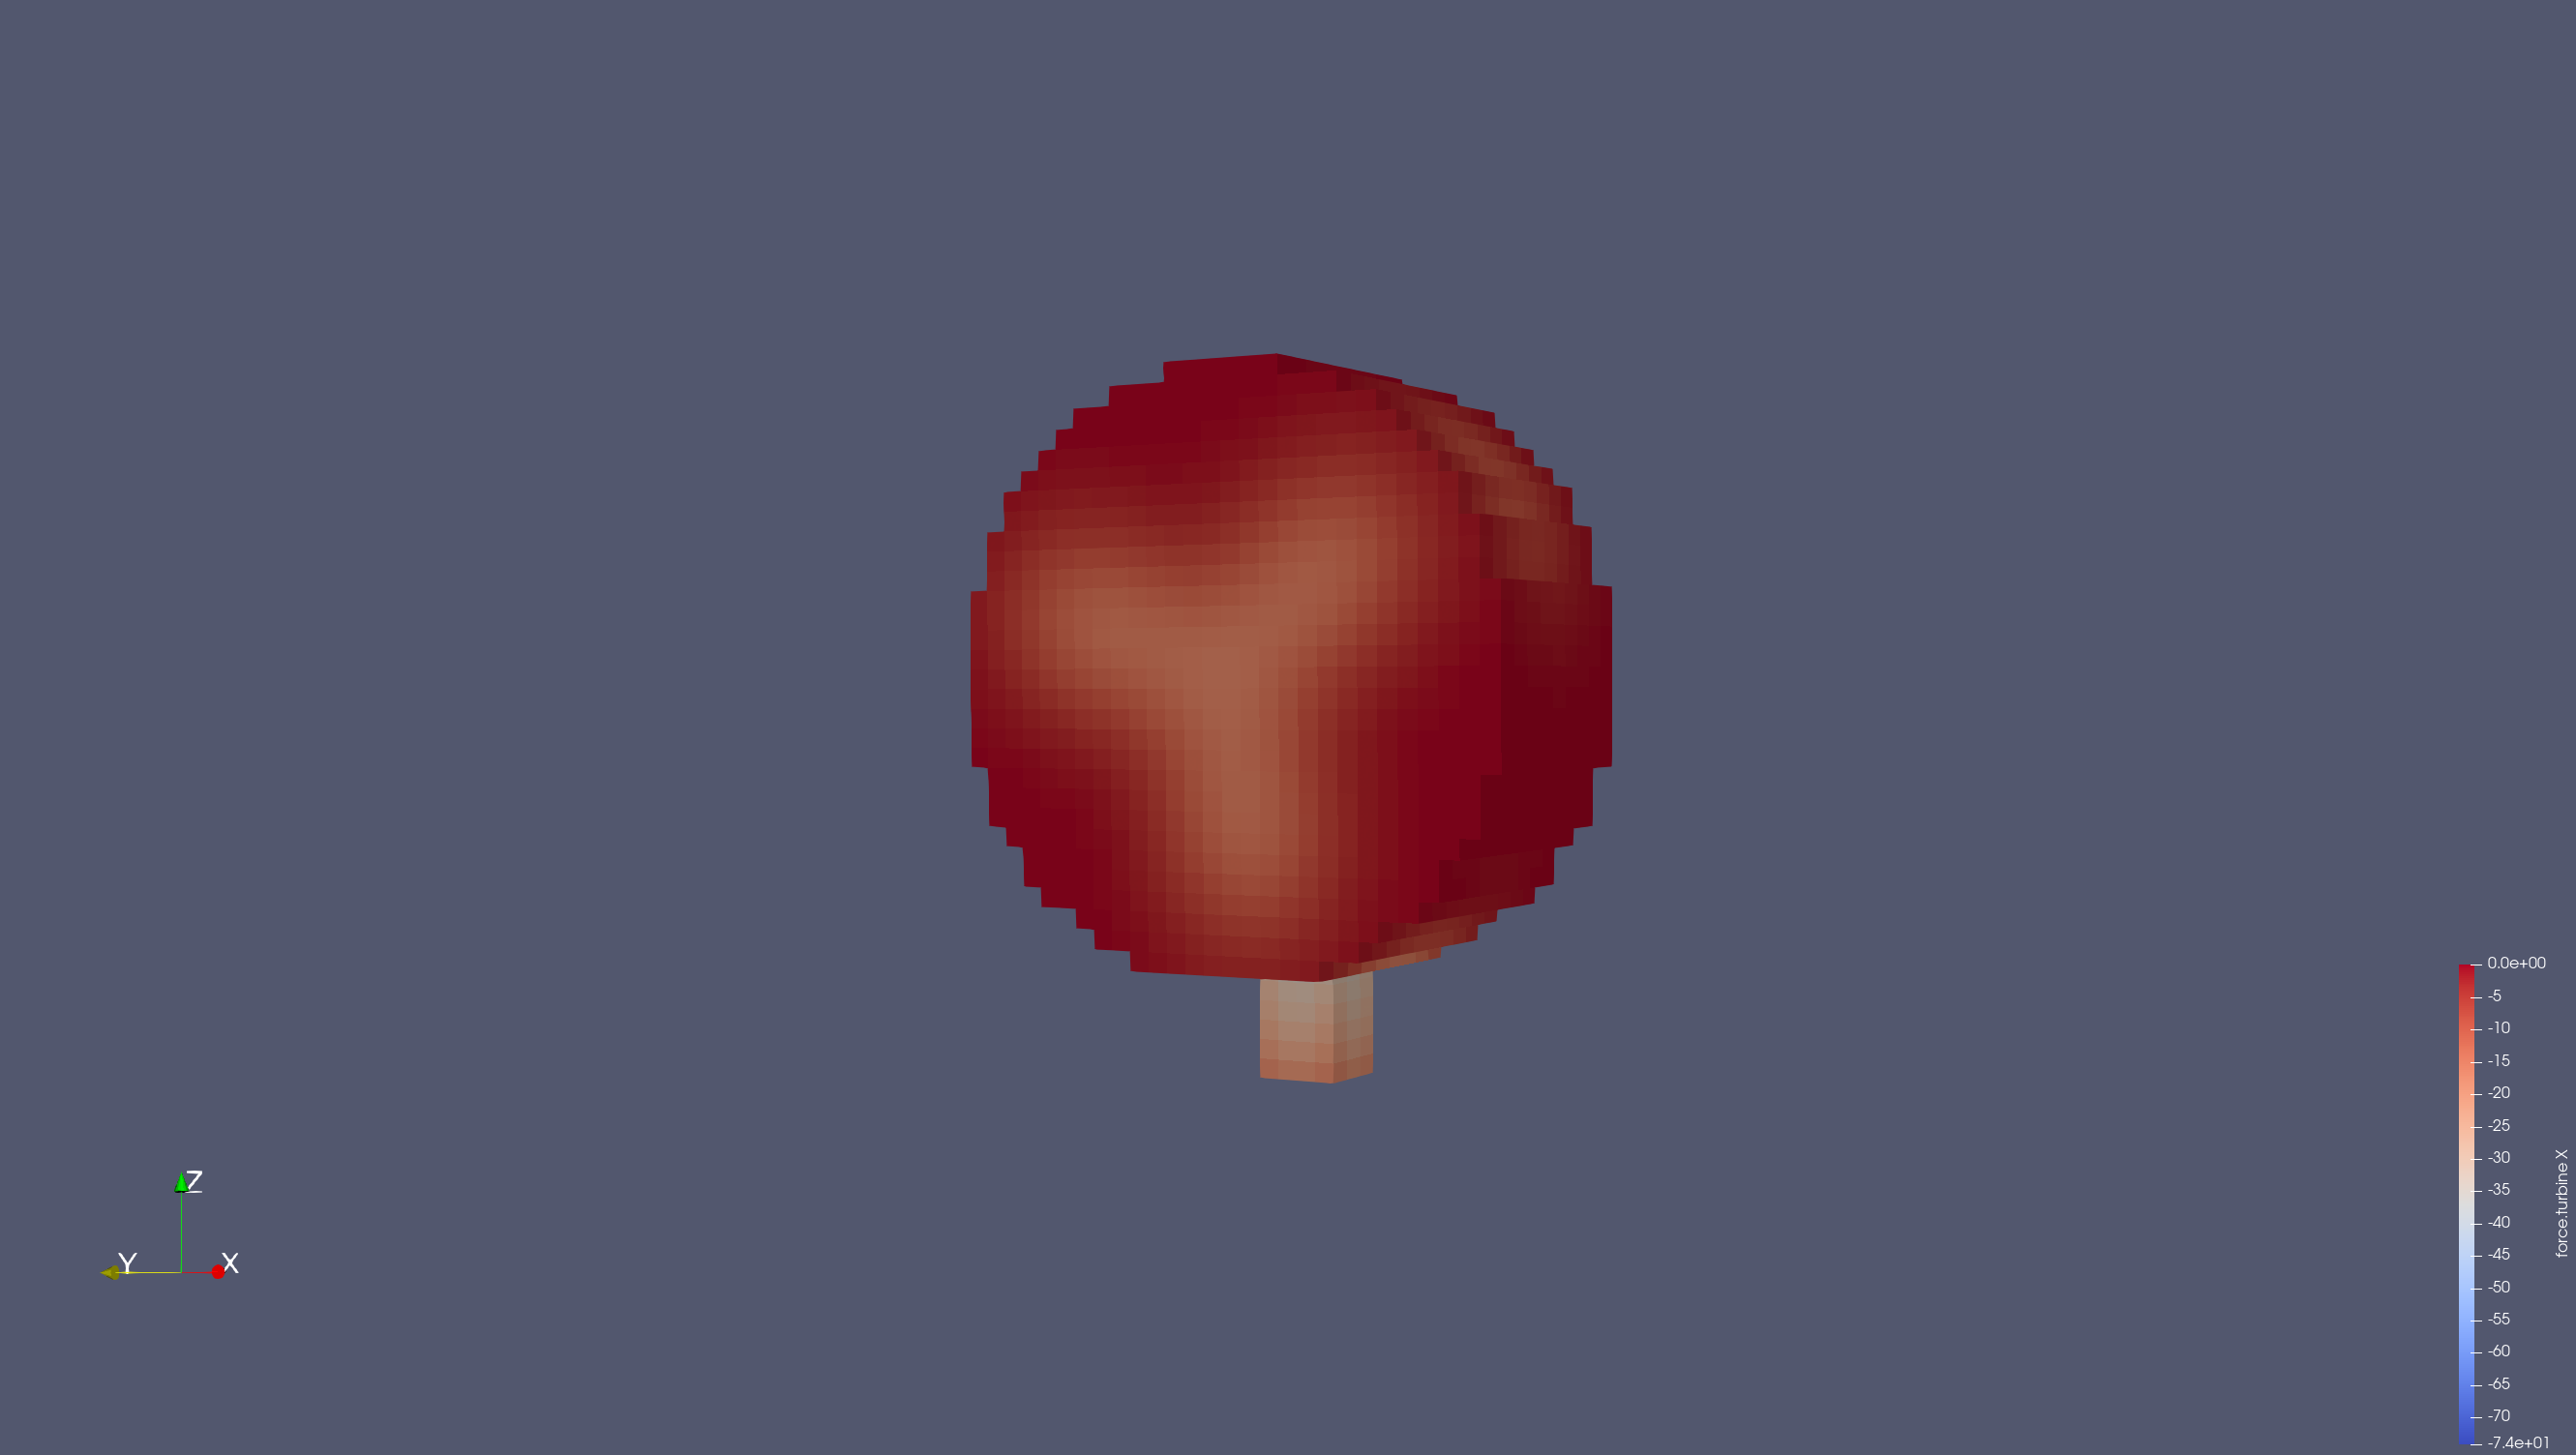
\includegraphics[width=\linewidth]{images/openfoam-turbine-mesh.png}
		\caption{Volume representation of the flow field immediately around the turbine in OpenFOAM}
		\label{fig:mesh:foam}
	\end{subfigure}
	\caption{Mesh differences between OpenFAST and the CFD solver OpenFOAM. OpenFAST uses the Actuator Line Model to represent blades and towers in the flow field, while OpenFOAM calculates the whole flow field.}
	\label{fig:mesh}
\end{figure*}

